%% ============================================================
%%  Beamer slides — Extension v5 for production model
%%  Supervisor discussion deck
%%  Compile: pdflatex extension_v5_slides.tex (twice)
%% ============================================================
\documentclass[10pt,aspectratio=169]{beamer}
\usetheme{default}
\usecolortheme{dove}
\useinnertheme{rectangles}
\setbeamertemplate{navigation symbols}{}
\setbeamertemplate{footline}[frame number]

\usepackage{booktabs}
\usepackage{array}
\usepackage{graphicx}
\graphicspath{{../05-modelling-production-data/figures/v5/}{../05-modelling-production-data/figures/}{figures/}}
\usepackage{amsmath, amssymb, bm}
\usepackage{xcolor}

\definecolor{hlblue}{HTML}{08519c}
\definecolor{hlred}{HTML}{c0392b}
\definecolor{hlgold}{HTML}{b8860b}
\definecolor{hlgreen}{HTML}{1e8449}

\newcommand{\hl}[1]{{\color{hlblue}\textbf{#1}}}
\newcommand{\bad}[1]{{\color{hlred}#1}}
\newcommand{\good}[1]{{\color{hlgreen}#1}}
\newcommand{\new}[1]{{\color{hlgold}\textbf{#1}}}

\title{Extension of the RSA Production Model\\
\large Mechanism-level exploration and the $2\!\times\!2$ tradeoff}
\author{Hening Wang}
\date{2026-04-15}

\begin{document}

% ====================================================================
\begin{frame}
\titlepage
\end{frame}

% ====================================================================
\begin{frame}{Where we start: the paper-reported model}
\small
Incremental recursive speaker, hierarchical per-participant $\alpha$ offsets. Theory-driven: minimal parameters with clear motivation.

\vspace{0.5em}
\hl{The $2\!\times\!2$ story (memo \S1):}
\begin{center}
\begin{tabular}{lrrrrr}
\toprule
Model & ELPD LOO & $\Delta$ ELPD & dSE & $\Delta$/dSE & $p$\\
\midrule
\hl{Inc.\ recursive} & \hl{$-7180$} & $0$ & --- & --- & ---\\
Inc.\ static        & $-7199$ & $-19$ & 1.84  & $-10.28$ & $<.001$\\
Global static       & $-7626$ & $-446$ & 40.27 & $-11.08$ & $<.001$\\
Global recursive    & $-7628$ & $-448$ & 40.69 & $-11.02$ & $<.001$\\
\bottomrule
\end{tabular}
\end{center}

\vspace{0.3em}
\begin{itemize}\itemsep0.2em
  \item \hl{Speaker architecture dominates}: incremental $\gg$ global ($\Delta/$dSE $\approx 11$).
  \item \hl{Semantic regime within incremental}: recursive $>$ static ($\Delta/$dSE $= 10.28$).
  \item \hl{Semantic regime within global}: null (global recursive slightly \emph{worse}).
\end{itemize}
\end{frame}

% ====================================================================
\begin{frame}{But: the fit is poor}
\small
Production data = categorical utterance choice among 15 types, in 9 conditions $\times$ 2 sharpness levels.

\vspace{0.3em}
\begin{itemize}\itemsep0.2em
  \item \bad{$R^2 = 0.346$} on the 90 (condition $\times$ utterance) cells.
  \item \bad{L1 aggregate residual $= 3.17$} across cells with empirical $\geq 2\%$.
  \item Lapse $\varepsilon = 0.22$ --- nearly a quarter of responses treated as uniform noise.
\end{itemize}

\vspace{0.5em}
\hl{Seven systematic misfits (memo \S5.3):}
\begin{center}
\footnotesize
\begin{tabular}{lll rrr}
\toprule
Condition & Sharpness & Utterance & Emp & Model & $\Delta$\\
\midrule
colour-sufficient & high & C    & .716 & .403 & $-.313$\\
size-sufficient   & low  & SF   & .365 & .081 & $-.284$\\
colour-sufficient & low  & C    & .628 & .402 & $-.225$\\
both-necessary    & low  & C    & .009 & .222 & $+.214$\\
size-sufficient   & high & SFC  & .022 & .211 & $+.189$\\
both-necessary    & high & C    & .000 & .175 & $+.175$\\
size-sufficient   & low  & SFC  & .032 & .187 & $+.155$\\
\bottomrule
\end{tabular}
\end{center}
\end{frame}

% ====================================================================
\begin{frame}{Diagnosis (memo \S5.3)}
Residuals decompose along two independent axes.

\vspace{0.5em}
\textbf{1.~Context-dependence of 1-word C:}
\begin{itemize}\itemsep0.1em
  \item Under-predicted by $\sim.25$--$.31$ in colour-sufficient contexts
  \item Over-predicted by $\sim.18$--$.21$ in both-necessary contexts
  \item No single $\alpha_C$ can fix both.
\end{itemize}

\vspace{0.5em}
\textbf{2.~Length residuals show saturation, not level shift:}
\begin{itemize}\itemsep0.1em
  \item 2-word (SF) under-predicted by $\sim.28$ in blurred size-sufficient
  \item 3-word (SFC) over-predicted by $\sim.17$ in size-sufficient
  \item No monotone change to a linear $\gamma$ fixes both.
\end{itemize}

\vspace{0.5em}
\hl{These diagnostics motivate the mechanism track.}
\end{frame}

% ====================================================================
\begin{frame}{Extension timeline (dc subset, $N = 3196$)}
\small
Conditions \texttt{erdc, zrdc, brdc} --- size $\times$ colour distinguishing, form redundant.
Three \texttt{relevant\_property} values inside: \texttt{first} (size-alone-sufficient),
\texttt{both} (both needed), \texttt{second} (colour-alone-sufficient).

\vspace{0.8em}
\begin{center}
\renewcommand{\arraystretch}{1.15}
\begin{tabular}{llll}
\toprule
Step & Mechanism & Parameters & Rationale\\
\midrule
ext-v1  & per-dim $\alpha$, $\gamma$, $\varepsilon$           & $\alpha_D,\alpha_C,\alpha_F,\gamma,\varepsilon$ & dim-salience asymmetry \\
v5a     & condition-gated colour boost                       & $\lambda_C$ & Pechmann 89; Rubio-Fern\'andez 16 \\
v5b     & saturating length bias                             & $\gamma_1,\gamma_2$ & overspec not monotone in length \\
v5 (F1) & + csuff length offsets                             & $\delta\gamma_1,\delta\gamma_2$ & bare-C when colour identifies \\
v5 (C1) & + canonical-order penalty                          & $\mu_\mathrm{nc}$ & Sproat 91; Cinque 94; Scott 02 \\
v5 (F2) & + sharpness-dependent length                       & $\eta_1,\eta_2$ & overspec more common under blur \\
\bottomrule
\end{tabular}
\end{center}

\vspace{0.5em}
\textbf{Flag correction:} \texttt{COLOUR\_SUFFICIENT\_CONDITIONS}
was first $(ercf, zrcf, brcf)$. Corrected to $(ercf, zrdc)$ --- only
conditions where colour alone identifies the target.
\end{frame}

% ====================================================================
\begin{frame}{Attempt 1: ext-v1 (already in memo \S4.1)}
Per-dimension $\alpha$ + explicit $\gamma$ + lapse $\varepsilon$.

\vspace{0.5em}
\begin{center}
\begin{tabular}{lrr}
\toprule
& ELPD & vs baseline\\
\midrule
baseline & $-7157$ & 0 \\
\hl{ext-v1}  & \hl{$-6387$} & \hl{$+770$} \\
\bottomrule
\end{tabular}
\quad
\begin{tabular}{lrr}
\toprule
& $R^2$ & L1\\
\midrule
baseline  & .35 & 3.17 \\
\hl{ext-v1}   & .60 & 3.17 \\
\bottomrule
\end{tabular}
\end{center}

\vspace{0.5em}
$\alpha_D = 6.94, \alpha_C = 1.84, \alpha_F = 1.88, \gamma = 2.32, \varepsilon = 0.22$.

\vspace{0.5em}
\hl{But:} seven memo \S5.3 misfits persist; $\varepsilon = 0.22$ uncomfortably high.
\end{frame}

% ====================================================================
\begin{frame}{Attempt 2a: $\lambda_C$ alone (v5a)}
Step-0 logit boost for \textbf{C} when \texttt{is\_colour\_sufficient} = 1.

\vspace{0.5em}
\begin{center}
\begin{tabular}{lrrr}
\toprule
& ELPD & $\Delta$ vs ext-v1 & $\lambda_C$ posterior\\
\midrule
ext-v1 & $-6387$ & 0 & --- \\
\hl{v5a}    & \hl{$-6265$} & \hl{$+122$}  & \hl{3.4} (95\% CI 2.8--4.0) \\
\bottomrule
\end{tabular}
\end{center}

\vspace{0.5em}
\begin{itemize}\itemsep0.2em
  \item Strong positive $\lambda_C$: colour gets extra first-step pull in colour-sufficient trials.
  \item \good{second/sharp C}: emp $.716$, was $.403$, now $.55$.
  \item \bad{CF still too high in second conditions}: boost spreads to C-initial compounds (\texttt{CF, CDF}). Not enough by itself.
\end{itemize}
\end{frame}

% ====================================================================
\begin{frame}{Attempt 2b: saturating $\gamma$ alone (v5b)}
Replace linear $\gamma \cdot k$ with $\gamma_1 \,\mathbb{I}[k \geq 1] + \gamma_2\,\mathbb{I}[k \geq 2]$.

\vspace{0.5em}
\begin{center}
\begin{tabular}{lrr}
\toprule
& ELPD & $\Delta$ vs ext-v1\\
\midrule
ext-v1 & $-6387$ & 0 \\
v5b    & $-6381$ & \bad{$+6$} \\
\bottomrule
\end{tabular}
\end{center}

\vspace{0.5em}
\bad{Essentially no improvement without $\lambda_C$.}

\vspace{0.5em}
The two mechanisms are synergistic: $\gamma$-saturation only matters after C-initial mass is correctly apportioned.
\end{frame}

% ====================================================================
\begin{frame}{Attempt 3: F1 --- condition-dependent length (v5 with $\delta\gamma$)}
Let the length bias \emph{shrink} on colour-sufficient trials
($\gamma_{1,\mathrm{eff}} = \gamma_1 + \delta\gamma_1 \cdot$ \texttt{is\_csuff}).

\vspace{0.5em}
\begin{center}
\begin{tabular}{lrrr}
\toprule
& ELPD & $\Delta$ vs ext-v1 & notes\\
\midrule
ext-v1 & $-6387$ & 0 & \\
v5a    & $-6265$ & $+122$ & $\lambda_C$ only \\
\hl{v5 (F1)} & \hl{$-5933$} & \hl{$+454$} & $\lambda_C + \delta\gamma$  \\
\bottomrule
\end{tabular}
\end{center}

\vspace{0.5em}
Posteriors: $\lambda_C = 5.0$, $\gamma_1 = 2.56$, $\gamma_2 = 0.92$, $\delta\gamma_1 = -1.89$, $\delta\gamma_2 = -3.51$, $\varepsilon = 0.16$.

\vspace{0.5em}
\hl{Effective $\gamma$ on colour-sufficient trials}: $0.67, -2.59$ --- 3-word heavily penalised, short utterances favoured.
$R^2 = .67$, L1 $= 2.70$.

\vspace{0.5em}
\bad{Remaining puzzle:} model still over-predicts \texttt{DC} and \texttt{DFC}, under-predicts \texttt{DCF} in both-necessary and first-conditions.
\end{frame}

% ====================================================================
\begin{frame}{Attempt 4: C1 --- canonical-ordering penalty}
Add $\mu_\mathrm{nc} \cdot \mathbb{I}[\text{utterance violates size} < \text{colour} < \text{form}]$.\\
Non-canonical set: \texttt{CD, CDF, CFD, DFC, FD, FDC, FC, FCD}.

\vspace{0.5em}
\begin{center}
\begin{tabular}{lrrr}
\toprule
& ELPD & $\Delta$ vs ext-v1 & notes\\
\midrule
v5 (F1) & $-5933$ & $+454$ & $\lambda_C + \delta\gamma$ \\
\hl{v5 (C1)} & \hl{$-5323$} & \hl{$+1063$} & \hl{$+ \mu_\mathrm{nc}$} \\
\bottomrule
\end{tabular}
\end{center}

\vspace{0.5em}
\hl{$\mu_\mathrm{nc} = -5.07$} --- speakers strongly prefer canonical English ordering.
\\[0.2em]
$\varepsilon$ drops to $0.10$.

\vspace{0.5em}
$R^2 = .91$, L1 $= 1.34$.

\vspace{0.3em}
\hl{7 of 8 user-flagged cells fixed}:
\texttt{DCF, DF, DC, DFC, C} residuals largely resolved. \\
\bad{Side-effect:} on \texttt{first/sharp}, bare \texttt{D} under-predicted ($.082$ vs emp $.269$) and \texttt{DF} over-predicted.
\end{frame}

% ====================================================================
\begin{frame}{Attempt 5: F2 --- sharpness-dependent length}
Add $\eta_1, \eta_2$ offsets active on \texttt{is\_sharp} trials.

\vspace{0.5em}
\begin{center}
\begin{tabular}{lrrr}
\toprule
& ELPD & $\Delta$ vs ext-v1 & $R^2$\\
\midrule
v5 (C1) & $-5323$ & $+1063$ & $.91$ \\
\hl{v5 (F2)} & \hl{$-5294$} & \hl{$+1093$} & \hl{$.94$} \\
\bottomrule
\end{tabular}
\end{center}

\vspace{0.5em}
Posteriors: $\eta_1 = -0.61$, $\eta_2 = -0.34$ (both informatively negative).\\
Effective $\gamma$ on sharp: $1.71, 1.24$ vs blurred: $2.32, 1.58$.

\vspace{0.5em}
$\varepsilon$ stays at $0.10$; 0 divergences throughout; all $\hat R \leq 1.02$.

\vspace{0.5em}
\hl{Stubborn residual:} \texttt{first/sharp D} still under-predicted (.269 vs .102). Likely strategy heterogeneity (some participants say bare \texttt{D}, others hedge with \texttt{F}).
\end{frame}

% ====================================================================
\begin{frame}{Final v5 (F2) parameters}
\small
\begin{center}
\begin{tabular}{lllc}
\toprule
Parameter & Prior & Posterior mean (95\% CI) & $\hat R$\\
\midrule
$\alpha_D$           & HalfN(5)    & (hier.\ w/ $\delta_p$)                 & $\leq 1.01$\\
$\alpha_C$           & HalfN(5)    & (hier.)                                 & $\leq 1.01$\\
$\alpha_F$           & HalfN(5)    & (hier.)                                 & $\leq 1.01$\\
$\lambda_C$          & N(0,1)      & $3.09$ (2.67, 3.55)                     & 1.00\\
$\gamma_1$           & N(0,1)      & $2.32$ (2.16, 2.49)                     & 1.00\\
$\gamma_2$           & N(0,1)      & $1.58$ (1.43, 1.74)                     & 1.01\\
$\delta\gamma_1$     & N(0,1)      & $-2.16$ (-2.33, -1.97)                  & 1.00\\
$\delta\gamma_2$     & N(0,1)      & $-0.58$ (-1.21, +0.04)                  & 1.00\\
$\eta_1$             & N(0,1)      & $-0.61$ (-0.77, -0.43)                  & 1.00\\
$\eta_2$             & N(0,1)      & $-0.34$ (-0.51, -0.15)                  & 1.00\\
$\mu_\mathrm{nc}$    & N(0,1)      & $-5.08$ (-5.61, -4.56)                  & 1.01\\
$\log\beta$          & N(0,0.5)    & $-0.17$                                 & 1.00\\
$\varepsilon$        & Beta(1,50)  & $0.10$ (0.09, 0.12)                     & 1.00\\
$\tau$               & HalfN(0.2)  & $0.62$ (0.51, 0.73)                     & 1.00\\
\bottomrule
\end{tabular}
\end{center}
\end{frame}

% ====================================================================
\begin{frame}{PPC barplot --- baseline vs ext-v1 vs v5 (F2)}
\vspace{-0.5em}
\begin{center}
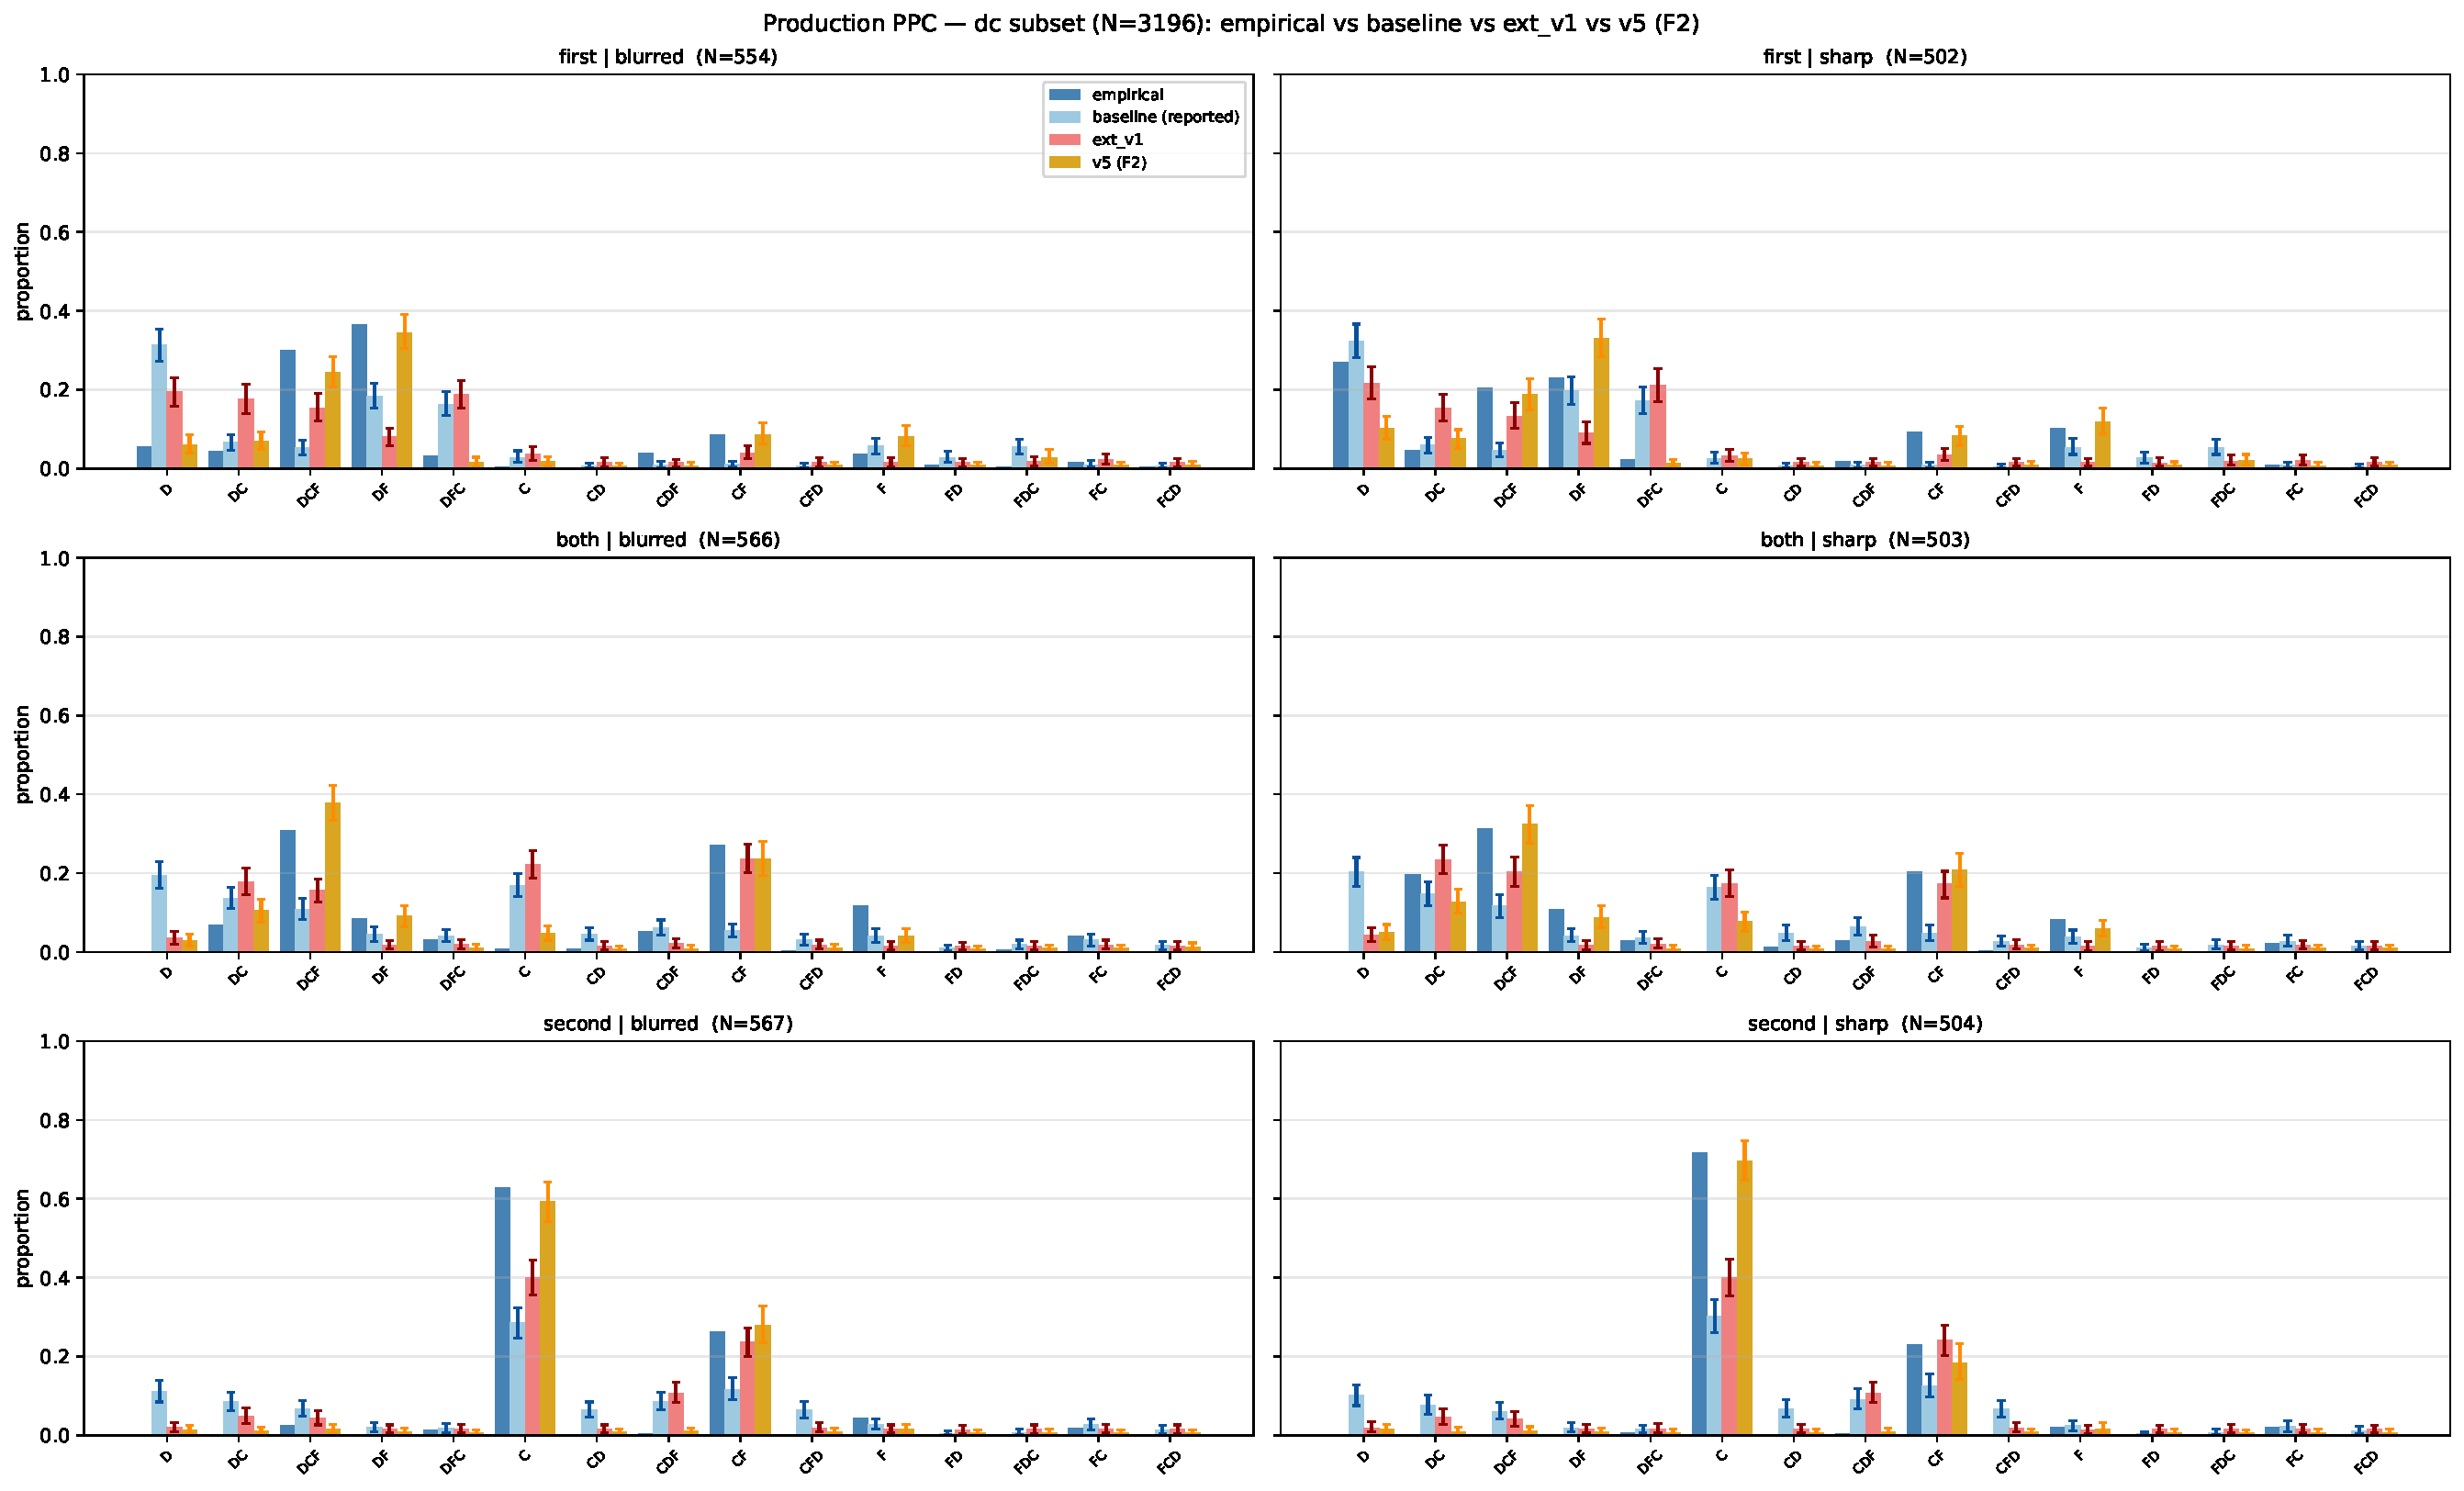
\includegraphics[width=0.98\linewidth]{production_ppc_barplot_v5_dc_F2.pdf}
\end{center}
\vspace{-0.3em}
\footnotesize{Rows: \texttt{relevant\_property} (first / both / second). Cols: sharpness.}
\end{frame}

% ====================================================================
\begin{frame}{Correlation --- predicted vs empirical ($n = 90$)}
\vspace{-0.5em}
\begin{center}
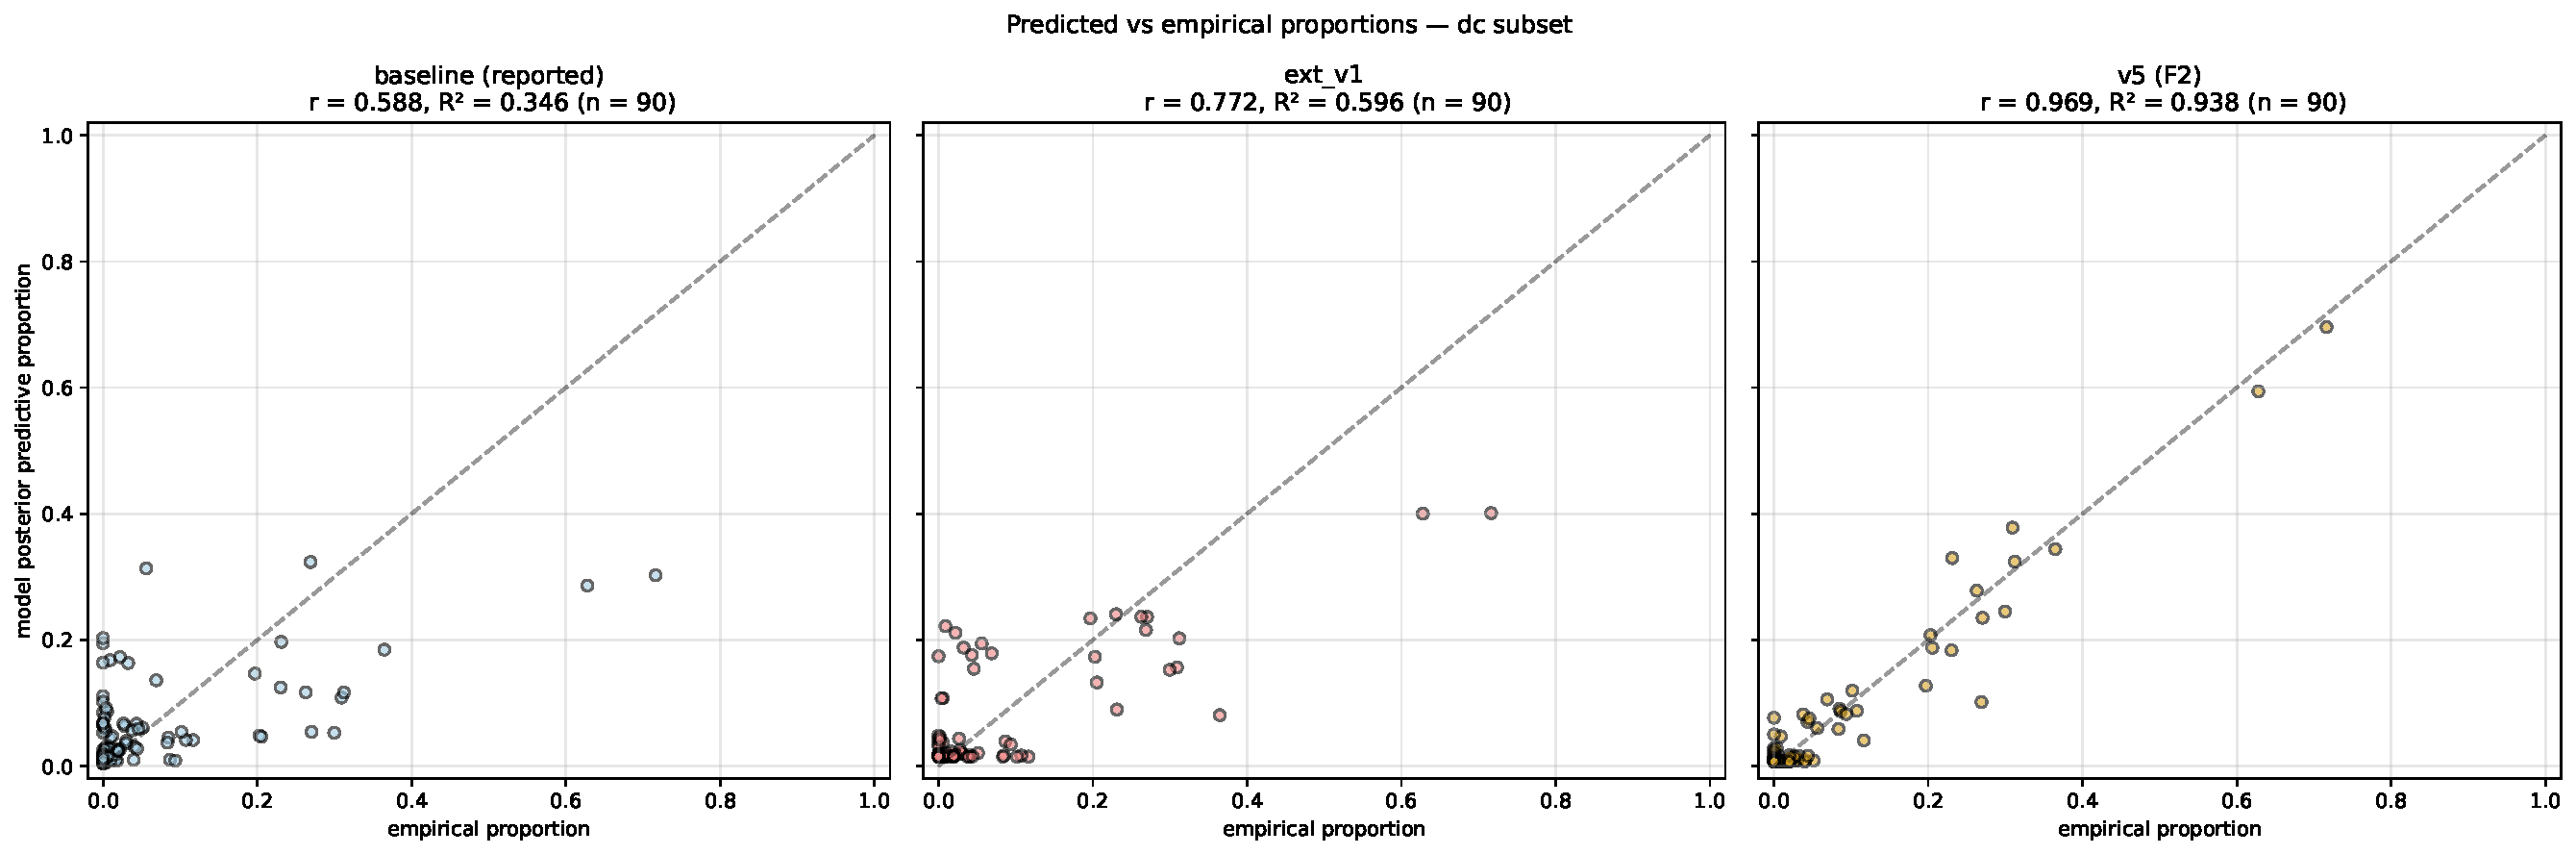
\includegraphics[width=0.98\linewidth]{production_correlation_v5_dc_F2.pdf}
\end{center}
\vspace{-0.3em}
\footnotesize{$R^2$ climbs: baseline $.35$, ext-v1 $.60$, \hl{v5 (F2) $.94$}.}
\end{frame}

% ====================================================================
\begin{frame}{The $2\!\times\!2$ question: does the paper story survive?}
We re-ran the $2\!\times\!2$ (speaker architecture $\times$ semantics regime) with F2 mechanisms in all four cells, then again with freely-sampled parameters in the global cells.

\vspace{0.8em}
Three parameterisations to compare:
\begin{enumerate}\itemsep0.3em
  \item \hl{Paper-reported (memo \S1)}: minimal, theory-driven.
  \item \hl{F2-fixed globals}: global cells use $\gamma/\delta\gamma/\eta/\mu_\mathrm{nc}$ fixed at incremental-recursive posterior means (memo \S5.1 convention).
  \item \hl{F2-full globals}: every parameter sampled freely in every cell. Fairest comparison.
\end{enumerate}
\end{frame}

% ====================================================================
\begin{frame}{$2\!\times\!2$: paper-reported}
\begin{center}
\begin{tabular}{l|rr|r}
\toprule
          & recursive & static & $\Delta$(rec$-$sta) \\
\midrule
incremental & $-7180$ & $-7199$ & \hl{$+19$} ($\Delta/$dSE $= 10.28$) \\
global      & $-7628$ & $-7626$ & $-2$ (null) \\
\midrule
$\Delta$(inc$-$glb) & $+448$ & $+427$ & \\
$\Delta/$dSE        & $11.02$ & $11.08$ & \\
\bottomrule
\end{tabular}
\end{center}

\vspace{0.8em}
\hl{Paper narrative:}
\begin{itemize}\itemsep0.2em
  \item Architecture dominates: inc $\gg$ glb, $\Delta/$dSE $\approx 11$.
  \item Recursive semantics helps incremental a lot, does \emph{not} help global.
  \item Diff-in-diff $= +21$ (inc benefits more from rec).
\end{itemize}
\end{frame}

% ====================================================================
\begin{frame}{$2\!\times\!2$: F2 with fixed global parameters}
\begin{center}
\begin{tabular}{l|rr|r}
\toprule
             & recursive & static & $\Delta$(rec$-$sta) \\
\midrule
incremental   & $-5294$ & $-5297$ & $+2.80$ ($\Delta/$dSE $= 2.22$, marginal) \\
global (fixed)& $-5600$ & $-5619$ & \hl{$+19.15$} ($\Delta/$dSE $= 6.99$) \\
\midrule
$\Delta$(inc$-$glb) & $+306$ & $+323$ & \\
$\Delta/$dSE        & $10.51$ & $11.03$ & \\
\bottomrule
\end{tabular}
\end{center}

\vspace{0.8em}
\begin{itemize}\itemsep0.2em
  \item Architecture still dominant ($\Delta/$dSE $\approx 10.5$).
  \item \bad{Interaction has flipped}: rec now helps global, not incremental.
  \item But global's length parameters are \emph{fixed at inc values} --- not a fair test.
\end{itemize}
\end{frame}

% ====================================================================
\begin{frame}{$2\!\times\!2$: F2 with fully-sampled globals (fair)}
\begin{center}
\begin{tabular}{l|rr|r}
\toprule
            & recursive & static & $\Delta$(rec$-$sta) \\
\midrule
incremental & $-5294$ & $-5297$ & $+2.80$ ($\Delta/$dSE $= 2.22$) \\
global (full) & $-5357$ & $-5365$ & $+8.25$ ($\Delta/$dSE $= 3.82$) \\
\midrule
$\Delta$(inc$-$glb) & $+63$ & $+69$ & \\
$\Delta/$dSE        & \hl{$3.18$} & \hl{$3.48$} & \\
\bottomrule
\end{tabular}
\end{center}

\vspace{0.8em}
\hl{Key changes vs paper-reported:}
\begin{itemize}\itemsep0.2em
  \item Architecture effect $\Delta/$dSE: $11 \to 3.2$ (\bad{$\sim\!1/3$ of paper's}).
  \item Regime-within-inc $\Delta/$dSE: $10.28 \to 2.22$ (\bad{$\sim\!1/5$ of paper's}).
  \item Regime-within-glb: $0 \to 3.82$ (\new{appears, modestly}).
  \item Diff-in-diff: $+21 \to +5.45$ (same direction flipped, small magnitude).
\end{itemize}
\end{frame}

% ====================================================================
\begin{frame}{Side-by-side}
\small
\begin{center}
\begin{tabular}{lccc}
\toprule
                             & Paper        & F2-fixed & \hl{F2-full} \\
\midrule
$R^2$ (all cells)            & $.35$      & $.94$ & $.94$ \\
L1 residual                  & $3.17$    & $1.22$   & $1.22$ \\
Lapse $\varepsilon$          & $0.22$      & $0.10$ & $0.10$ \\
\midrule
Arch effect $\Delta/$dSE     & $\pm 11$    & $\pm 10.5$ & $\pm 3.2$ \\
Regime $|$inc $\Delta/$dSE   & $10.28$     & $2.22$ & $2.22$ \\
Regime $|$glb $\Delta/$dSE   & $\approx 0$ & $6.99$ & $3.82$ \\
Interaction (diff-in-diff)   & $+21$       & $-16$ & $+5.45$ \\
\midrule
Rec helps\ldots              & incremental & global (artefact) & slightly global \\
\bottomrule
\end{tabular}
\end{center}
\end{frame}

% ====================================================================
\begin{frame}{The tradeoff}
\begin{columns}[t]
\begin{column}{0.48\textwidth}
\textbf{\color{hlblue}Theory track (paper)}
\begin{itemize}\itemsep0.2em
  \item Minimal, motivated mechanisms
  \item Clear $2\!\times\!2$ interaction
  \item \bad{Poor group-level fit ($R^2 = .35$)}
  \item \bad{Seven large misfits in \S5.3}
  \item Lapse absorbs unexplained structure
\end{itemize}
\end{column}

\begin{column}{0.48\textwidth}
\textbf{\color{hlgold}Mechanism track (F2)}
\begin{itemize}\itemsep0.2em
  \item Rich, but each term literature-grounded
  \item Excellent fit ($R^2 = .94$)
  \item All seven misfits resolved/improved
  \item Lapse halved ($0.22 \to 0.10$)
  \item \bad{Architecture signal shrinks to $\Delta/$dSE $= 3$}
  \item \bad{Regime-within-inc weakens to marginal}
\end{itemize}
\end{column}
\end{columns}

\vspace{1em}
\hl{Core tension.} Mechanisms designed to reduce residuals
explain variance that the paper's minimal parameterisation
attributed to \emph{architecture $\times$ regime}. The interaction survives
in reduced form.
\end{frame}

% ====================================================================
\begin{frame}{Two readings}
\small
\textbf{\color{hlblue}Reading I: mechanisms as rivals}

The paper's interaction was partly \emph{architectural sparsity fitting error structure}. Once the error is absorbed by explicit mechanisms (colour salience, canonical ordering, context-dependent length), the residual architectural signal is modest. The main claim must weaken.

\vspace{1em}
\textbf{\color{hlgold}Reading II: mechanisms as scaffolding}

$\lambda_C$, $\mu_\mathrm{nc}$, $\delta\gamma$, $\eta$ are \emph{implementations} of what context-updating $\times$ incremental architecture is \emph{supposed to do}. Of course adding them absorbs architectural signal --- they are the phenomena the architecture was indirectly capturing.

\vspace{1em}
\hl{Both are defensible. The choice shapes the paper's framing.}
\end{frame}

% ====================================================================
\begin{frame}{Four concrete decisions}
\begin{enumerate}\itemsep0.4em
  \item \textbf{Report v5 (F2) or keep the paper-reported model?}\\
  \small A middle path: main-text keeps the reported model; supplementary section shows F2 as mechanism-level refinement.

  \item \textbf{If we adopt F2, how do we frame the interaction?}\\
  \small Reading I softens. Reading II preserves. A referee will ask.

  \item \textbf{Adopt the corrected \texttt{COLOUR\_SUFFICIENT} flag $(ercf, zrdc)$?}\\
  \small Independent of the F2 decision. Probably yes --- the definition is simply more accurate.

  \item \textbf{Generalise beyond the dc subset?}\\
  \small Parallel runs on df and cf subsets would test whether F2 mechanisms are symmetric or colour-specific.
\end{enumerate}
\end{frame}

% ====================================================================
\begin{frame}{Open questions}
\small
\begin{itemize}\itemsep0.4em
  \item \textbf{Strategy heterogeneity.} $\varepsilon = 0.10$ is smaller than ext-v1's $0.22$ but non-zero. The \texttt{first/sharp} bare-\texttt{D} vs \texttt{DF} split looks like two participant sub-populations (minimum-description vs redundant-form). A mixture model is the natural next step.

  \item \textbf{Full-data ($N = 9586$) run.} Our early full-data run used the incorrect flag. A clean full-data F2 run would take $\sim\!15$ min on the GPU and complete the picture.

  \item \textbf{df and cf subsets.} Do the same mechanisms generalise? If a "form-sufficient" flag is needed, that would point to symmetric structure; if not, to colour-specificity.

  \item \textbf{LOO warnings.} All F2 \texttt{az.compare} outputs flagged \texttt{warning=True} (some Pareto $k > 0.7$). Differences reliable in direction, not in exact magnitude.
\end{itemize}
\end{frame}

% ====================================================================
\begin{frame}{Summary}
\small
\begin{itemize}\itemsep0.3em
  \item Paper-reported model: theory-driven, interpretable 2$\times$2 story, but $R^2 = .35$.
  \item Systematic residuals trace to three independent phenomena: \hl{colour salience}, \hl{canonical ordering}, \hl{condition-dependent length bias}.
  \item Adding all three (v5 F2) lifts fit to $R^2 = .94$ and lapse to $.10$ with 11 free population parameters, every one informative, 0 divergences.
  \item Re-running the $2\!\times\!2$ under F2 with all parameters sampled: architecture effect shrinks $\sim 3\times$, regime effect shrinks and partially flips direction.
  \item Two readings of the tradeoff; both defensible.
  \item Decision the paper needs: \hl{report F2, report paper-reported, or both?}
\end{itemize}

\vspace{1em}
\hl{Artefacts:} \footnotesize branch \texttt{feat/extension-v5},
spec at \texttt{docs/superpowers/specs/...},
plan at \texttt{docs/superpowers/plans/...},
synthesis at \texttt{10-writing/extension\_v5\_synthesis.md}.
\end{frame}

% ====================================================================
\begin{frame}{Thanks}
\centering
\vspace{2em}
\Large Questions and discussion.

\vspace{2em}
\normalsize
\begin{tabular}{ll}
\texttt{feat/extension-v5} & all changes, 15 commits \\
\texttt{10-writing/extension\_v5\_synthesis.md} & detailed write-up \\
\texttt{05-modelling-production-data/figures/v5/} & figures used above \\
\texttt{05-modelling-production-data/results/} & LOO + residual CSVs \\
\end{tabular}
\end{frame}

\end{document}
